\documentclass[11pt,handout,xcolor=pdftex,dvipsnames,table,mathserif,aspectratio=169]{beamer}
\usetheme{metropolis}
%\usetheme{Darmstadt}
%\usepackage{times}
%\usefonttheme{structurebold}

\usepackage[english]{babel}
%\usepackage[table]{xcolor}
\usepackage{amsmath}
\usepackage{pgf,pgfarrows,pgfnodes,pgfautomata,pgfheaps}
\usepackage{amsmath,amssymb,setspace}
\usepackage[latin1]{inputenc}
\usepackage[T1]{fontenc}
\usepackage{relsize}

%\usepackage[cache=false]{minted}
%\renewcommand{\MintedPygmentize}{/Users/christopherconlon/anaconda3/bin/pygmentize}

\usepackage[absolute,overlay]{textpos} 
\newenvironment{reference}[2]{% 
  \begin{textblock*}{\textwidth}(#1,#2) 
      \footnotesize\it\bgroup\color{red!50!black}}{\egroup\end{textblock*}} 

\DeclareMathSizes{10}{10}{6}{6} 


\title [Nonparametrics]{Nonparametrics and Local Methods: Polynomials}
\author{C.Conlon}
\institute{Applied Econometrics}
\date{\today}
\setbeamerfont{equation}{size=\tiny}
\begin{document}

\begin{frame}
\titlepage
\end{frame}

\begin{frame}{Polynomial Basis}
Again consider the following relationship:
\begin{align*}
y_i = f(x_i) + \epsilon_i
\end{align*}
One approach is to approximate $f(x_i)$ or $E[y_i | x_i]$ with a \alert{polynomial series}.
\begin{align*}
y_i = a_0  + a_1 x_i + a_2 x_i^2 + a_3 x_i^3+ \cdots+ a_M x_i^M + \varepsilon_i
\end{align*}
An important choice is to choose polynomial order $M$ (complexity)\\
Idea: we can approximate \alert{arbitrary (smooth) functions} $f(x_i)$ with a high-order polynomial.
\end{frame}

\begin{frame}{Polynomial Example}
Let's suppose we want to approximate the following function:
\begin{align*}
\frac{1}{3} \sin (2 x) \approx \frac{2}{3} x - \frac{4}{9} x^3 + \frac{4}{45} x^5 + O(x^7)
\end{align*}
This should be easy since we have a \alert{Taylor Expansion} that is polynomial in $x$ (also it is odd).
\end{frame}

\begin{frame}[fragile]{Polynomial Example}
\begin{columns}
\begin{column}{0.5\textwidth}
 \tiny
\begin{verbatim}
library(ggplot2)    

# set the seed to make the results reproducible.
set.seed(3)







#### simulate some data ####
# epsilon = random error term
epsilon <- 0.25*rnorm(100)
x       <- seq(from=1, to=5, length.out=100)
y       <- 1 +sin(x*2)/3 + epsilon





# visualize the data (with a polynomial best-fit line)
ggplot(data=NULL,aes(x, y)) + geom_point() + 
geom_smooth(method = "lm", formula = y ~ poly(x, 3,raw=T),color='maroon')+
geom_smooth(method = "lm", formula = y ~ poly(x, 5,raw=T),color='navy')+
geom_smooth(method = "lm", formula = y ~ poly(x, 17,raw=T),color='darkgreen')
\end{verbatim}
\end{column}
\begin{column}{0.5\textwidth}  %%<--- here
    \begin{center}
    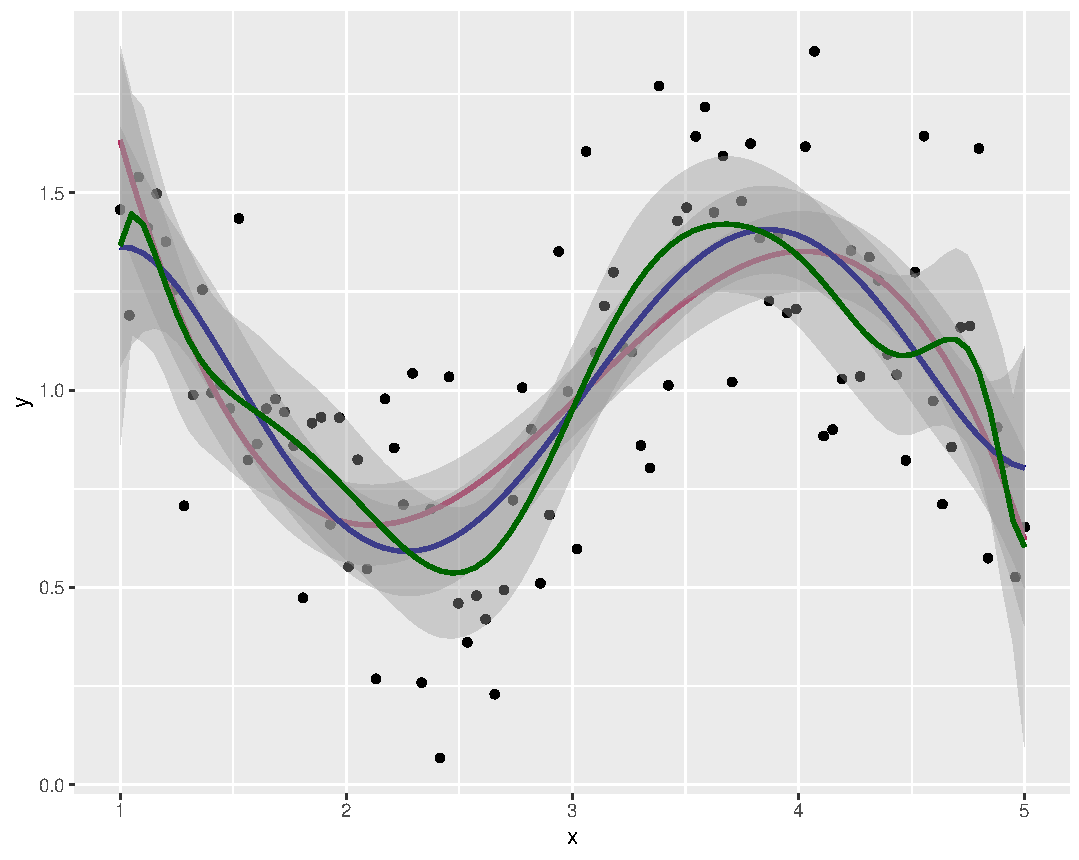
\includegraphics[width=\textwidth]{./resources/poly.pdf}
     \end{center}
\end{column}
\end{columns}
\end{frame}

\begin{frame}[fragile]{Polynomial Example}
\begin{itemize}
\item $M=5$ order polynomial should fit the data well (it does).
\item We are clearly \alert{overfitting} at $M=17$ since this doesn't look much like $y(x) = \sin(2x)/3 + \varepsilon$.
\item We used \alert{raw polynomials}: $x,x^2,x^3,\ldots$.
\item By default R uses \alert{orthogonal polynomials} when we drop \texttt{raw=TRUE}.\\
(More on these later)
\end{itemize}
\tiny 
\begin{verbatim}
# visualize the data (with a polynomial best-fit line)
ggplot(data=NULL,aes(x, y)) + geom_point() + 
geom_smooth(method = "lm", formula = y ~ poly(x, 3),color='maroon')+
geom_smooth(method = "lm", formula = y ~ poly(x, 5),color='navy')+
geom_smooth(method = "lm", formula = y ~ poly(x, 17),color='darkgreen')
\end{verbatim}
\end{frame}

\begin{frame}[fragile]{``Raw'' Polynomials}
\begin{columns}
\begin{column}{0.6\textwidth}
\tiny
\begin{verbatim}
                          Estimate Std. Error t value Pr(>|t|)
(Intercept)              -5.421717   8.009814  -0.677    0.500
poly(x, 6, raw = T)1  18.072018  20.371055   0.887    0.377
poly(x, 6, raw = T)2 -17.392013  20.363051  -0.854    0.395
poly(x, 6, raw = T)3   7.503790  10.288970   0.729    0.468
poly(x, 6, raw = T)4  -1.561290   2.786268  -0.560    0.577
poly(x, 6, raw = T)5   0.148442   0.385418   0.385    0.701
poly(x, 6, raw = T)6  -0.004826   0.021378  -0.226    0.822
\end{verbatim}

\begin{verbatim}
                          Estimate Std. Error t value Pr(>|t|)   
(Intercept)               45.71304   19.95109   2.291  0.02423 * 
poly(x, 7, raw = TRUE)1 -138.78101   59.74402  -2.323  0.02239 * 
poly(x, 7, raw = TRUE)2  177.80275   72.90420   2.439  0.01665 * 
poly(x, 7, raw = TRUE)3 -120.61050   47.13566  -2.559  0.01214 * 
poly(x, 7, raw = TRUE)4   46.52356   17.50188   2.658  0.00926 **
poly(x, 7, raw = TRUE)5  -10.21667    3.74637  -2.727  0.00765 **
poly(x, 7, raw = TRUE)6    1.18842    0.42965   2.766  0.00686 **
poly(x, 7, raw = TRUE)7   -0.05682    0.02044  -2.780  0.00658 **
\end{verbatim}
\end{column}
\begin{column}{0.4\textwidth}
\begin{itemize}
\item 6th order polynomial: nothing significant
\item 7th order polynomial: all terms significant (odd and even).
\item Totally different coefficients!
\item Both highly sensitive to small changes in $x_i$.
\end{itemize}
\end{column}
\end{columns}
\end{frame}


\begin{frame}[fragile]{``Orthogonal'' Polynomials}
\begin{columns}
\begin{column}{0.6\textwidth}
\tiny
\begin{verbatim}
                         Estimate Std. Error t value Pr(>|t|)    
(Intercept)               1.02278    0.02779  36.803  < 2e-16 ***
poly(x, 6, raw = FALSE)1  0.64772    0.27791   2.331  0.02193 *  
poly(x, 6, raw = FALSE)2  0.48158    0.27791   1.733  0.08643 .  
poly(x, 6, raw = FALSE)3 -2.47613    0.27791  -8.910 4.14e-14 ***
poly(x, 6, raw = FALSE)4 -0.16435    0.27791  -0.591  0.55571    
poly(x, 6, raw = FALSE)5  0.79114    0.27791   2.847  0.00543 ** 
poly(x, 6, raw = FALSE)6 -0.06273    0.27791  -0.226  0.82190    
\end{verbatim}

\begin{verbatim}
                         Estimate Std. Error t value Pr(>|t|)    
(Intercept)               1.02278    0.02684  38.111  < 2e-16 ***
poly(x, 7, raw = FALSE)1  0.64772    0.26837   2.414  0.01778 *  
poly(x, 7, raw = FALSE)2  0.48158    0.26837   1.794  0.07602 .  
poly(x, 7, raw = FALSE)3 -2.47613    0.26837  -9.227 9.68e-15 ***
poly(x, 7, raw = FALSE)4 -0.16435    0.26837  -0.612  0.54179    
poly(x, 7, raw = FALSE)5  0.79114    0.26837   2.948  0.00405 ** 
poly(x, 7, raw = FALSE)6 -0.06273    0.26837  -0.234  0.81569    
poly(x, 7, raw = FALSE)7 -0.74618    0.26837  -2.780  0.00658 ** 
\end{verbatim}
\end{column}
\begin{column}{0.4\textwidth}
\begin{itemize}
\item Odd terms are significant in both specifications
\item Coefficients appear stable (!)
\item Usually coefficients decline in (odd) polynomial order.
\item But very high dimensional polynomials will still \alert{overfit}.
\end{itemize}
\end{column}
\end{columns}
\end{frame}

\begin{frame}{Orthgonal Polynomials}
Consider an arbitrary basis:
\begin{align*}
y(x_i) = a_0 + \sum_{j=1}^M a_j b_j(x_i) + \varepsilon_i
\end{align*}
\begin{itemize}
\item $ b_j(x_i) = x_i^j$ (regular polynomials)
\item $\langle b_j(x),b_k(x)  \rangle=0$ for $j \neq k$ (orthogonal polynomials).
\item Lots of options: Chebyshev, Legendre, Fourier, Gram Schmidt (discuss later).
\end{itemize}
\end{frame}

\begin{frame}{What R does: Gram Schmidt}
Let $a_j = x^j$ (the raw polynomial) and then \alert{orthogonalize} as follows:
\begin{align*}
\hat{p}_{j}(x)&=a_{j}(x)-\sum_{k=0}^{j-1} p_{k}(x) \frac{p_{k} \cdot a_{j}}{p_{k} \cdot p_{k}}, \quad 
p(x)=\frac{\hat{p}(x)}{ \hat{p}(1)}
\end{align*}
\begin{itemize}
\item We are forming the \alert{residual} of $x^j$ on $(x^{j-1}, x^{j-2},\ldots, x, 1)$ (where each term has already been residualized).
\item Notice, we don't need to know $y_i$, we can simply residualized $x_i$ against powers of itself.
\item We could do this for any matrix $X$! (doesn't need to be powers of $x_i$).
\end{itemize}
\end{frame}


\begin{frame}{Orthogonal Polynomials}
\small
\begin{block}{General Case}
\begin{itemize}
\item Space: polynomials over domain $D$
\item Weighting function: $w(x) > $ (positive everywhere)
\item Inner product $\langle f,g \rangle = \int_D f(x) g(x) w(x) d x$
\item Polynomials are orthogonal wrt to $w(x)$ IFF 
\begin{eqnarray*}
\langle \phi_i, \phi_j \rangle = 0, \quad i \neq j
\end{eqnarray*}
\item Can compute orthogonal polynomials using recurrence formulas
\begin{eqnarray*}
\phi_0(x) &=& 1\\
\phi_1(x) &=& x \\
\phi_{k+1}(x) &=& (a_{k+1} x + b_k) \phi_k(x) + c_{k+1} \phi_{k-1}(x)
\end{eqnarray*}
\end{itemize}
\end{block}
\end{frame}

\begin{frame}{Chebyshev Polynomials}
\small
\begin{itemize}
\item Can compute orthogonal polynomials using recurrence formulas
\item $[a,b] = [-1,1]$ and $w(x) = (1-x^2)^{-1/2}$
\item $T_n(x) = \cos(n \cos^{-1} x)$
\item Recursive Definition 
\begin{eqnarray*}
T_0(x) &=& 1\\
T_1(x) &=& x\\
T_{n+1}(x) &=& 2x T_n(x) - T_{n-1}(x)
\end{eqnarray*}
\end{itemize}
\begin{block}{General Intervals}
\begin{itemize}
\item Most problems aren't on the $[-1,1]$ interval so we need a COV
\begin{eqnarray*}
y = -1 + 2 \frac{x-a}{b-a}
\end{eqnarray*}
\item Polynomials $\phi_i^{*}(x) \equiv \phi_i (-1 + 2 \frac{x-a}{b-a})$ are orthogonal over $x \in[a,b]$ with respect to the weight $w^{*}(x) \equiv (-1 + 2 \frac{x-a}{b-a})$ iff the $\phi_i(y)$ are orthogonal over $y\in[-1,1]$ wrt $w(y)$.
\end{itemize} 
\end{block}
\end{frame}

\begin{frame}{Chebyshev Approximation Algorithm}
\small
\begin{enumerate}
\item Compute the $m \geq n+1$ Chebyshev nodes on $[-1,1]$
\begin{eqnarray*}
z_k = -\cos \left ( \frac{2k-1}{2m} \pi \right) , \quad k=1,\ldots,m
\end{eqnarray*}
\item Adjust the nodes to $[a,b]$ interval
\begin{eqnarray*}
x_k = (z_k + 1)\left(\frac{b-a}{2} \right) + a , \quad k=1,\ldots,m
\end{eqnarray*}
\item Evaluate $f$ at the nodes $w_k = f(x_k)$ for $ k=1,\ldots,m$
\item Compute the coefficients $a_i$ to get the approximation $p(x)$
\begin{eqnarray*}
a_i = \frac{\sum_{k=1}^m w_k T_i(z_k)}{\sum_{k=1}^m  T_i(z_k)^2}, \quad
p(x) = \sum_{i=0}^n a_i T_i \left( 2 \frac{x-a}{b-a} -1 \right) 
\end{eqnarray*}
\end{enumerate}
\end{frame}

\begin{frame}{Minimax Approximation}
\begin{itemize}
\item Data: $(x_i,y_i)$, $i=1,\ldots,n$
\item Objective: $L^{\infty}$ fit
\begin{eqnarray*}
\min_{\beta \in R^m} \max_{i} \| y_i - f(x_i; \beta) \|
\end{eqnarray*}
\item Difficult to do (minimax problems are non-convex)
\item Chebyshev Approximation satisfies this property, for $C^2,C^3$ functions but doesn't get $f'(x)$ right!
\end{itemize}
\begin{theorem}
Suppose $f: [-1,1] \rightarrow R$ is $C^k$ for some $k \geq 1$, and let $I_n$ be the degree $n$ polynomial interpolation of $f$ based at the zeroes of $T_{n+1}(x)$ then
\begin{eqnarray*}
\tiny
\| f - I_n \|_{\infty} \leq \left(\frac{2}{\pi}  \log(n+1) + 1 \right) \frac{(n-k)!}{n!} \left ( \frac{\pi}{2}\right)^k  \left ( \frac{b-a}{2}\right)^k \| f^{(k)} \|_{\infty}
\end{eqnarray*}
\end{theorem}
\end{frame}

\begin{frame}{Recap: Polynomials}
\begin{align*}
y(x_i) = a_0 + \sum_{j=1}^M a_j b_j(x_i) + \varepsilon_i
\end{align*}
\begin{itemize}
\item Thus far have looked at \alert{global polynomial approximations}.
\item Global: basis $b_j(x)$ and coefficients $a_j$ are the same for any value of $x$.
\item Can choose polynomial order with \alert{cross validation}, later we will explore \alert{penalization}.
\item Special case of \alert{sieve estimators}: we let the order $M \rightarrow \infty$ as $n \rightarrow \infty$.
\end{itemize}

\end{frame}


\begin{frame}{Splines}
Splines are piecewise interpolating functions
\begin{definition} 
A function $s(x)$ on $[a,b]$ is a spline of order $n$ IFF
\begin{enumerate}
\item $s$ is $C^{n-2}$ on $[a,b]$ and 
\item there is a grid of points (nodes) $a = x_0 < x_1 < \cdots < x_m = b$ such that $s(x)$ is a polynomial of degree $n-1$ on each subinterval $[x_i, x_{i+1}]$, $i = 0,\ldots,m-1$
\end{enumerate}
\end{definition}
Second order plane is piecewise linear.\\
We usually use cubic splines.
\end{frame}


\begin{frame}{Splines}
Cubic Splines
\begin{itemize}
\item Lagrange data set $(x_i,y_i)$ for $i=0,\ldots n$.
\item Nodes: the $x_i$ are the nodes of the spline
\item Functional form $s(x) = a_i + b_i x + c_i x^2 + d_i x^3$ on $[x_{i-1},x_i]$
\item Unknowns $4n$ unknown coefficients
\item $2n$ interpolation and continuity conditions:
\begin{eqnarray*}
y_i &=& a_i + b_i x_i + c_i x_i^2 + d_i x_i^3 \quad i=1,\dots, n\\
y_i &=& a_{i+1} + b_{i+1} x_i + c_{i+1} x_i^2 + d_{i+1} x_i^3 \quad i=0,\ldots, n-1
\end{eqnarray*}
\item $2n - 2$ conditions from $C^2$ at the interior for $i=1,\ldots,n-1$
\begin{eqnarray*}
b_i + 2c_i x_i + 3 d_i x_i^2  &=& b_{i+1} + 2 c_{i+1} x_i + 3 d_{i+1}x_i^2\\ 
2c_i + 6d_i x_i &=& 2c_{i+1} + 6d_{i+1} x_i
\end{eqnarray*}
\end{itemize}
\end{frame}


\begin{frame}{Side Conditions}
We have $4n-2$ linear equations and $4n$ unknowns we need two side conditions to identify the system
\begin{itemize}
\item Natural spline: $s''(x_0) = s''(x_n) = 0$ minimizes the total curvature $\int_{x_0}^{x_n} s''(x)^2 dx$
\item Hermite spline: $s'(x_0) = y_0'$ and $s'(x_n) = y_n'$ (with extra data)
\item Secant Hermite: $s'(x_0) = \frac{s(x_1) - s(x_0)}{x_1-x_0}$ , $s'(x_n) = \frac{s(x_n) - s(x_{n-1})}{x_n-x_{n-1}}$
\item Solvers are built in to packages like MATLAB (check documentation for which method).
\end{itemize}
\end{frame}


\begin{frame}{Shape Issues}
\begin{figure}[htbp]
\begin{center}
\includegraphics[height=2in]{./resources/spline.pdf}
\label{default}
\end{center}
\end{figure}
\begin{itemize}
\item Concave (monotone) data may lead to non concave (non monotone) approximations
\item Shape problems stabilize VFI.
\end{itemize}
\end{frame}

\begin{frame}{Schumaker Procedure (Shape Preserving Splines)}
\begin{enumerate}
\item Take level (and maybe slope) data at nodes $x_i$
\item Add intermediate nodes $z_i^{+} \in [x_i,x_{i+1}]$
\item Run quadratic spline with nodes at the $x$ and $z$ nodes which interpolate data and preserves shape
\item Schumaker formulas tell you how to choose the $z$ and spline coefficient
\item Detail in Judd and in companion paper (Judd and Solnick)
\end{enumerate}
\end{frame}


\end{document}